\documentclass{article}
\usepackage{paralist}
\usepackage{graphicx}
\usepackage{fancyhdr}
\usepackage{datetime}


\begin{document}

\title{Interactive Graphics Report\\
		Homework 1}
\author{Jean-Pierre Richa}
\date{May 2018}
\maketitle
\section {Introduction}
\textbf {In this report, we are going to explain the work done for the interactive graphics first homework.
The homework contained 7 questions, which we are going to see and explain their implementation in details.}

\section {Implementation}
\textbf{In this section, we are going to address each problem and discuss its implementation. The code pieces will not be shown in the report, because it is scattered in multiple files. For that, all of the code is already commented using the question number it belongs to.}


\begin{enumerate}
\item Add a button that changes the direction of the current rotation:

In this question we were supposed to add a button to switch the direction of rotation on the current rotating axis, so I had to create a button in the HTML file, create a flag in the javascript file and put a condition(if statement) in the render function and tell it to rotate in the positive or the negative direction of rotation around the current axis.

\item Move the transformations matrices to the Javascript application:

Here we had to move the transformation matrices from the HTML to the javascript file, so the modelViewMatrix and projectionMatrix are computed in the application and then transferred to the 
shader. In order to do this, I had to discard the rx, ry, and rz matrices and use the function "rotate" from mv.js, I calculated the rotations in the javascript file, and then sent the final modelViewMatrix including all the multiplications of the rotations into the HTML file.

\item Include a scaling and a translation Matrix and control them with sliders:

This was feasible through creating 2 sliders, 1 for the translation and 1 for the scaling, sending their values to the javascript file, calculating the translate and scale matrices functions taken from the mv.js file, and then multiplying them by the modelViewMatrix. After that, I sent the modelViewMatrix back to the HMTL file. The scaling values will be all the same, so scale x, y, and z will have the same value(it was required in the given), so the cube sides will be proportional.

\item Define an orthographic projection with the planes near and far controlled by sliders:

To define the orthographic projection, we need to use the \textbf{\underline {ortho}} function from the \textbf{\underline{mv.js}} class to declare the projectionMatrix. As for the modelViewMatrix, it should be declared using the \textbf{\underline {lookAt}} function that define the distance and angle(position) from which we are looking at the object(the cube in our case). After the declaration, we do the multiplications we explained in questions 2 and 3 and then the projectionMatrix, and modelViewMatrix, should be sent to the HTML file. I also created the near and far sliders for changing the distance and position from where we are looking at the cube. To change the position, I took the value from the slider and calculated it in the \textbf{\underline {ortho}} function that contains the near and far attributes.

\item Define a perspective projection, and switch between orthographic and perspective projection:

Here we had to not only define a perspective projection, and switch between orthographic and perspective projection using a button, but the slider for near and far should also work for both projections.
The projectionMatrix is the perspective now, so we define it and then we do what we did in steps 2 and 3. I also defined a button that switches between the 2 projections using a flag in the javascript file 

\item Introduce a light source:

Here I had to define the \textbf{light position}, \textbf{ambient}, \textbf{diffuse}, and \textbf{specular} as well as the \textbf{materials}, and \textbf{shininess}. I then calculated the ambient, diffuse and specular products, which will be sent to the vertex shader, or fragment shader (depending on what we need to calculate, as we will see in the last point) to calculate the different colors, depending on whether the light is hitting the vertices or not.

\item Implement both the Gouraud and the Phong shading models, with a button switching between
them:

At this point we almost reached the end of the homework. In order to understand how to implement this, we need to understand the difference between gouraud and phong shading. the only difference is that gouraud shading is calculated in the vertex shader, and phong shading is calculated in the fragment shader. The vertex shader is less computationally expansive. On the contrary, the fragment shader is more computationally expansive, which means that the fragment shader will give more realistic results. here we need the vertex shader and the fragment shader to interact, so we need to send information from the vertex shader to the fragment shader. In order to do this, we should assign the information to a varying variable, but we can't send information from the fragment shader to the vertex shader, because the vertex is executed before the fragment. Summarising, the phong shading will look more realistic than the gouraud shading.

\section {Conclusion}
\textbf{Summarising, it was interesting to work on different kinds of implementations. Going through the code and the different ways of implementing the same thing gives us a very good knowledge about the variety of calculations that can be done. For example, the implementation of \textit{\underline{almost}} all the points can be done also in the HTML file, and not only in the JS file. Looking down at the screenshots, we can see all the sliders, the color of the cube(of course the cube is rotating), and the difference between gouraud and phong shading.}

\begin{figure}[!ht]
\centering
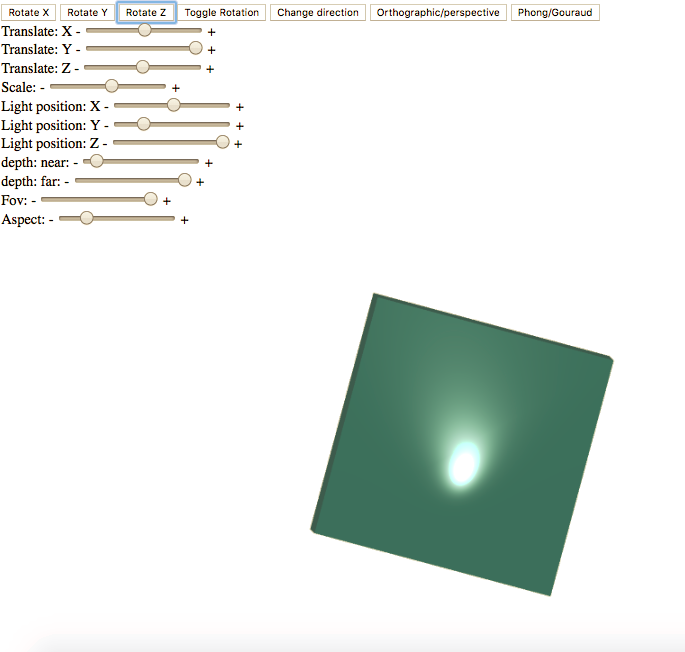
\includegraphics[scale=0.40]{HW1}
\caption{Phong}
\label{fig:fig1}
\end{figure}

\begin{figure}[!ht]
\centering
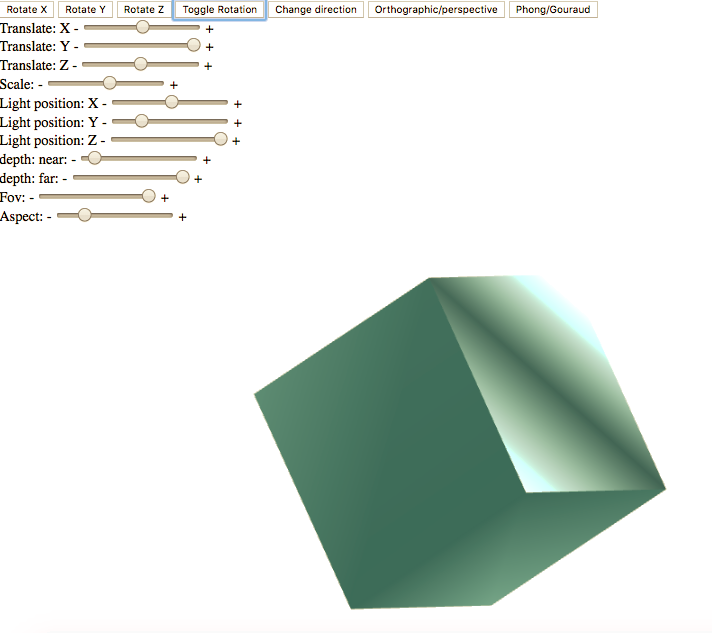
\includegraphics[scale=0.30]{HW2}
\caption{Gouraud}
\label{fig:fig1}
\end{figure}

\end{enumerate}
\end{document}